\chapter{Lab 3: Advanced molecular calculations}
\label{chap:lab_advanced_molecules}

\section{Topics covered in this lab}
This lab covers molecular QMC calculations with wavefunctions of increasing sophistication.  All of the trial wavefunctions are initially generated with the GAMESS code.  Topics covered include:
\begin{itemize}
  \item{Generating single-determinant trial wavefunctions with GAMESS (HF and DFT)}
  \item{Generating multideterminant trial wavefunctions with GAMESS (CISD, CASCI, and SOCI)}
  \item{Optimizing wavefunctions (Jastrow factors and CSF coefficients) with QMC}
  \item{DMC time step and walker population convergence studies}
  \item{Systematic progressions of Jastrow factors in VMC}
  \item{Systematic convergence of DMC energies with multideterminant wavefunctions}
  \item{Influence of orbitals basis choice on DMC energy}
  %\item{Influence of orbitals basis choice on rate of multi-determinant DMC convergence}
\end{itemize}

\section{Lab directories and files}
\footnotesize
\begin{verbatim}
labs/lab3_advanced_molecules/exercises
│    
├── ex1_first-run-hartree-fock    - basic work flow from Hatree-Fock to DMC
│   ├── gms                        - Hatree-Fock calculation using GAMESS
│   │   ├── h2o.hf.inp               - GAMESS input
│   │   ├── h2o.hf.dat               - GAMESS punch file containing orbitals
│   │   └── h2o.hf.out               - GAMESS output with orbitals and other info
│   ├── convert                    - Convert GAMESS wavefunction to QMCPACK format
│   │   ├── h2o.hf.out               - GAMESS output
│   │   ├── h2o.ptcl.xml             - converted particle positions
│   │   └── h2o.wfs.xml              - converted wave function
│   ├── opt                        - VMC optimization
│   │   └── optm.xml                 - QMCPACK VMC optimization input
│   ├── dmc_timestep               - Check DMC timestep bias
│   │   └── dmc_ts.xml               - QMCPACK DMC input
│   └── dmc_walkers                - Check DMC population control bias
│       └── dmc_wk.xml               - QMCPACK DMC input template
│   
├── ex2_slater-jastrow-wf-options - explore jastrow and orbital options
│   ├── jastrow                    - Jastrow options
│   │   ├── 12j                      - no 3-body Jastrow
│   │   ├── 1j                       - only 1-body Jastrow
│   │   └── 2j                       - only 2-body Jastrow
│   └── orbitals                   - Orbital options
│       ├── pbe                      - PBE orbitals
│       │   └── gms                    - DFT calculation using GAMESS
│       │      └── h2o.pbe.inp          - GAMESS DFT input
│       ├── pbe0                     - PBE0  orbitals
│       ├── blyp                     - BLYP  orbitals
│       └── b3lyp                    - B3LYP orbitals
│       
├── ex3_multi-slater-jastrow
│   ├── cisd                      - CISD wave function
│   │   ├── gms                     - CISD calculation using GAMESS
│   │   │   ├── h2o.cisd.inp           - GAMESS input
│   │   │   ├── h2o.cisd.dat           - GAMESS punch file containing orbitals
│   │   │   └── h2o.cisd.out           - GAMESS output with orbitals and other info
│   │   └── convert                 - Convert GAMESS wavefunction to QMCPACK format
│   │      └── h2o.hf.out             - GAMESS output
│   ├── casci                     - CASCI wave function
│   │   └── gms                     - CASCI calculation using GAMESS
│   └── soci                      - SOCI wave function
│       ├── gms                     - SOCI calculation using GAMESS
│       ├── thres0.01               - VMC optimization with few determinants
│       └── thres0.0075             - VMC optimization with more determinants
│   
└── pseudo
    ├── H.BFD.gamess             - BFD pseudopotential for H in GAMESS format
    ├── O.BFD.CCT.gamess         - BFD pseudopotential for O in GAMESS format
    ├── H.xml                    - BFD pseudopotential for H in QMCPACK format
    └── O.xml                    - BFD pseudopotential for H in QMCPACK format
\end{verbatim}
\normalsize

\section{Exercise \#1: Basics}

The purpose of this exercise is to show how to generate wavefunctions for QMCPACK
using GAMESS and to optimize the resulting wavefunctions using VMC. This will be
followed by a study of the time step and walker population dependence of DMC energies.
The exercise will be performed on a water molecule at the equilibrium geometry.


\subsection{Generation of a Hartree-Fock wavefunction with GAMESS}

From the top directory, go to ``\texttt{ex1\_first-run-hartree-fock/gms}.'' This directory contains an input
file for a HF calculation of a water molecule using BFD ECPs and the corresponding
cc-pVTZ basis set. The input file should be named: “h2o.hf.inp.” Study the input
file. See Section~\ref{sec:lab_adv_mol_gamess}, ``Appendix A: GAMESS input" for a more detailed description of the
GAMESS input syntax. However, there will be a better time to do this soon, so we recommend
continuing with the exercise at this point. After you are done, execute
GAMESS with this input and store the standard output in a file named ``h2o.hf.output.''
Finally, in the ``convert'' folder, use \texttt{convert4qmc} to generate the QMCPACK \texttt{particleset} and \texttt{wavefunction} files. It
is always useful to rename the files generated by \texttt{convert4qmc} to something meaningful
since by default they are called \texttt{sample.Gaussian-G2.xml} and \texttt{sample.Gaussian-G2.ptcl.xml}.
In a standard computer (without cross-compilation), these tasks can be accomplished by
the following commands.
\begin{lstlisting}[style=SHELL]
cd ${TRAINING TOP}/ex1_first-run-hartree-fock/gms
jobrun_vesta rungms h2o.hf 
cd ../convert
cp ../gms/h2o.hf.output
jobrun_vesta convert4qmc -gamessAscii h2o.hf.output -add3BodyJ
mv sample.Gaussian-G2.xml h2o.wfs.xml
mv sample.Gaussian-G2.ptcl.xml h2o.ptcl.xml
\end{lstlisting}
\noindent

%Due to the particular requirements of Vesta these executions can not be performed on
%the login nodes, they must be performed in the compute nodes. In order to accomplish
%this, we must make a submission script with the appropriate commands and submit it to
%the batch system. Two submission scripts have been provided, one for the GAMESS 
%execution called submit gamess.csh and one for the submission of convert4qmc, with a similar
%descriptive name. Study these input files. (In this and all other exercises, you will need
%to make all submission scripts executables with the command chmod u+x script.csh.)
%When you are ready, start by submitting the GAMESS execution to the batch system
%using ``./script gamess.csh'' (This script calls the GAMESS run script, which itself calls
%qsub. Do not attempt to submit this specific script with qsub). 
The HF energy of the
system is -16.9600590022 Ha. To search for the energy in the output file quickly, you can
use 
\begin{shade}
grep "TOTAL ENERGY =" h2o.hf.output
\end{shade}
%When the calculation completes,
%submit the execution of the converter using ``qsub submit convert.csh'' (all QMCPACK execution 
%scripts will be submitted with qsub). This is a good time to review section B, which
%contains a description on the use of the converter.
As the job runs on VESTA, it is a good time to review Section~\ref{sec:lab_adv_mol_convert4qmc}, ``Appendix B: convert4qmc," which contains a description on the use of the converter.


\subsection{Optimize the wavefunction}
When execution of the previous steps is completed, there should be two new
files called \texttt{h2o.wfs.xml} and \texttt{h2o.ptcl.xml}. Now we will use VMC to optimize the 
Jastrow parameters in the wavefunction.  From the top directory, go to
``\texttt{ex1\_first-run-hartree-fock/opt}.'' Copy the xml files generated in the previous step
to the current directory. This directory should already contain a basic QMCPACK input
file for an optimization calculation (\texttt{optm.xml}) %and a submission script (submit.csh). 
Open \texttt{optm.xml} with your favorite text editor and modify the name of the files that contain the
\texttt{wavefunction} and \texttt{particleset} XML blocks. These files are included with the commands:
\begin{lstlisting}[style=QMCPXML]
<include href=ptcl.xml/>
<include href=wfs.xml/>
\end{lstlisting}
(the particle set must be
defined before the wavefunction). The name of the particle set and wavefunction files should now be \texttt{h2o.ptcl.xml}
and \texttt{h2o.wfs.xml}, respectively. Study both files and submit when you are ready. Notice that the
location of the ECPs has been set for you; in your own calculations you have to make
sure you obtain the ECPs from the appropriate libraries and convert them to QMCPACK
format using ppconvert. While these calculations finish is a good time to study Section~\ref{sec:lab_adv_mol_opt_appendix}, ``Appendix C: Wavefunction optimization XML block," which contains a review
of the main parameters in the optimization XML block.  The
previous steps can be accomplished by the following commands:
\begin{shade}
cd ${TRAINING TOP}/ex1_first-run-hartree-fock/opt
cp ../convert/h2o.wfs.xml ./
cp ../convert/h2o.ptcl.xml ./
# edit optm.xml to include the correct ptcl.xml and wfs.xml
jobrun_vesta qmcpack optm.xml
\end{shade}

Use the analysis tool \texttt{qmca} to analyze the results of the calculation. Obtain the VMC
energy and variance for each step in the optimization and plot it using your favorite program.
Remember that \texttt{qmca} has built-in functions to plot the analyzed data.
\begin{shade}
qmca -q e *scalar.dat -p
\end{shade}

\begin{figure}
\begin{center}
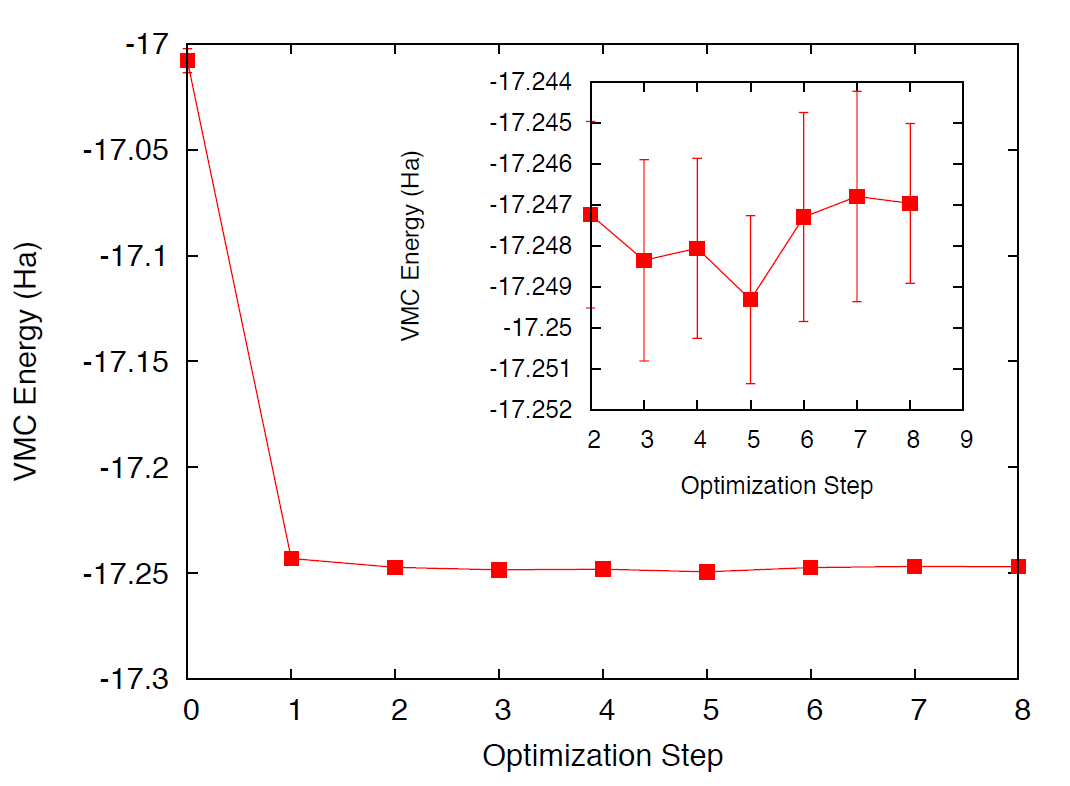
\includegraphics[trim = 0mm 0mm 0mm 0mm, clip,width=0.75\columnwidth]{./figures/lab_advanced_molecules_opt_conv.png}
\end{center}
\caption{VMC energy as a function of optimization step.}
\label{fig:lam_opt_conv}
\end{figure}

The resulting energy as a function of the optimization step should look qualitatively similar to Figure \ref{fig:lam_opt_conv}.
The energy should decrease quickly as a function of the number of optimization steps. After 6--8 steps, the energy should be converged to $\sim$2--3 mHa. To improve convergence,
we would need to increase the number of samples used during optimization (You can
check this for yourself later.). With optimized wavefunctions, we are in a position
to perform VMC and DMC calculations. The modified wavefunction files after each step
are written in a file named \texttt{ID.sNNN.opt.xml}, where ID is the identifier of the calculation
defined in the input file (this is defined in the project XML block with parameter “id”) and
NNN is a series number that increases with every executable xml block in the input file.


\subsection{Time-step study}
Now we will study the dependence of the DMC energy with time step. From the top directory, 
go to “\texttt{ex1\_first-run-hartree-fock/dmc\_timestep}.” This folder contains a basic XML input
file (\texttt{dmc\_ts.xml}) that performs a short VMC calculation and three DMC calculations
with varying time steps (0.1, 0.05, 0.01). Link the \texttt{particleset} and the last \texttt{optimization}
file from the previous folder (the file called \texttt{jopt-h2o.sNNN.opt.xml} with the largest value of
NNN). Rename the optimized \texttt{wavefunction} file to any suitable name if you wish (for example,
\texttt{h2o.opt.xml}) and change the name of the \texttt{particleset} and \texttt{wavefunction} files in the
input file. An optimized wavefunction can be found in the reference files (same location)
in case it is needed. %Using the submission script of the previous exercise as a base, create a
%submission script for this step and submit the run. Set the number of nodes to 32 (2 places
%must be changed), the number of threads to 16 and leave the number of tasks at 1.

The main steps needed to perform this exercise are:
\begin{lstlisting}[style=SHELL]
cd \$\{TRAINING TOP\}/ex1_first-run-hartree-fock/dmc_timestep
cp ../opt/h2o.ptcl.xml ./
cp ../opt/jopt-h2o.s007.opt.xml h2o.opt.wfs.xml
# edit dmc_ts.xml to include the correct ptcl.xml and wfs.xml
jobrun_vesta qmcpack dmc_ts.xml
\end{lstlisting}
While these runs complete, go to Section\ref{sec:lab_adv_mol_vmcdmc_appendix}, ``Appendix D: VMC and DMC XML block," and review the basic VMC and DMC input
blocks. Notice that in the current DMC blocks the time step is decreased as the number of blocks is increased. Why is this?

When the simulations are finished, use \texttt{qmca} to analyze the output files and plot the
DMC energy as a function of time step. Results should be qualitatively similar to those
presented in Figure \ref{fig:lam_dmc_timestep}; in this case we present more time steps with well converged results to
better illustrate the time step dependence. In realistic calculations, the time step must be
chosen small enough so that the resulting error is below the desired accuracy. Alternatively,
various calculations can be performed and the results extrapolated to the zero time-step
limit.


\begin{figure}
\begin{center}
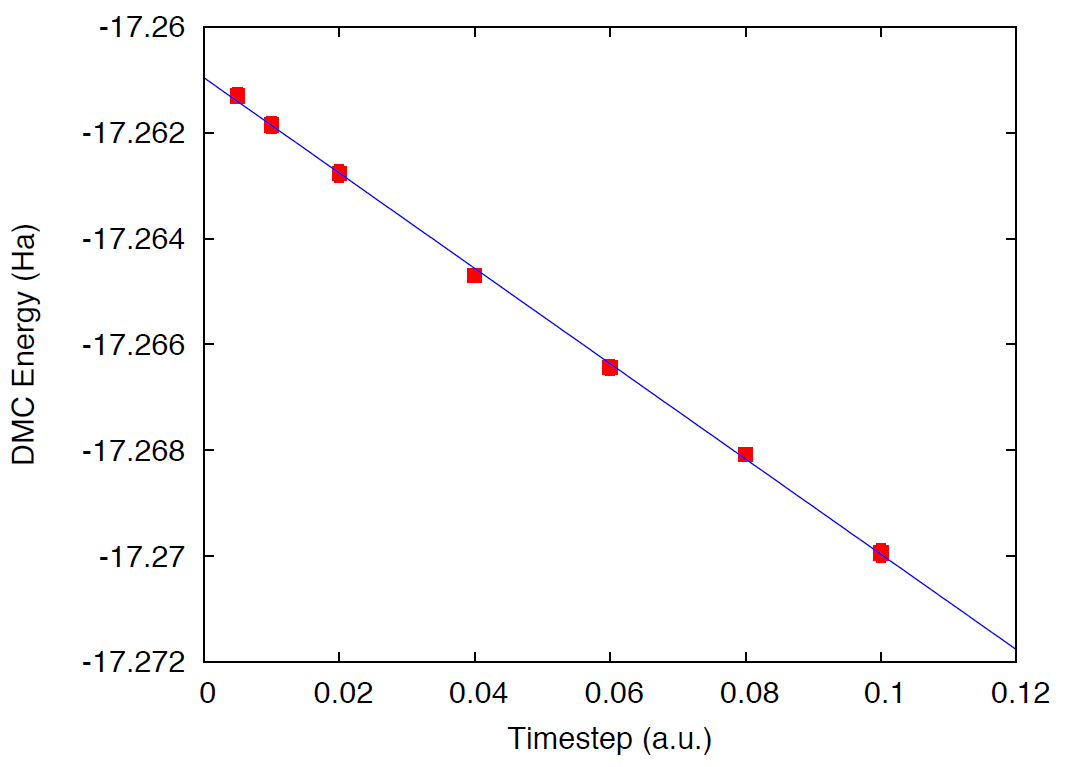
\includegraphics[trim = 0mm 0mm 0mm 0mm, clip,width=0.75\columnwidth]{./figures/lab_advanced_molecules_dmc_timestep.png}
\end{center}
\caption{DMC energy as a function of time step.}
\label{fig:lam_dmc_timestep}
\end{figure}


\subsection{Walker population study}
Now we will study the dependence of the DMC energy with the number of walkers in the
simulation. Remember that, in principle, the DMC distribution is reached in the limit of
an infinite number of walkers. In practice, the energy and most properties converge to high
accuracy with $\sim$100--1,000 walkers. The actual number of walkers needed in a calculation
will depend on the accuracy of the VMC wavefunction and on the complexity and size of
the system. Also notice that using too many walkers is not a problem; at worse it will be
inefficient since it will cost more computer time than necessary. In fact, this is the strategy
used when running QMC calculations on large parallel computers since we can reduce the
statistical error bars efficiently by running with large walker populations distributed across
all processors.

From the top directory, go to ``\texttt{ex1\_first-run-hartree-fock/dmc\_walkers}.'' Copy the
optimized \texttt{wavefunction} and \texttt{particleset} files used in the previous calculations to the current
folder; these are the files generated during step 2 of this exercise. An optimized \texttt{wavefunction} file can be found in the reference files (same location) in case it is needed. The directory
contains a sample DMC input file and submission script. Create three  directories named NWx,
with x values of 120,240,480, and copy the input file to each one. Go
to ``NW120,'' and, in the input file, change the name of the \texttt{wavefunction} and \texttt{particleset}
files (in this case they will be located one directory above, so use ``\texttt{../dmc\_timestep/h2.opt.xml},'' for
example); change the PP directory so that it points to one directory above; change ``targetWalkers'' to 120; and change the number of steps to 100, the time step
to 0.01, and the number of blocks to 400. Notice that ``targetWalkers'' is one way to set the desired (average) number of walkers in a DMC calculation. One can alternatively set ``samples'' in the \ixml{<qmc method="vmc"} block to carry over de-correlated VMC configurations as DMC walkers. For your own simulations, we generally recommend setting $\sim$2*(\#threads)
walkers per node (slightly smaller than this value).

The main steps needed to perform this exercise are
\begin{shade}
cd ${TRAINING TOP}/ex1_first-run-hartree-fock/dmc_walkers
cp ../opt/h2o.ptcl.xml ./
cp ../opt/jopt-h2o.s007.opt.xml h2o.opt.wfs.xml
# edit dmc_wk.xml to include the correct ptcl.xml and wfs.xml and 
#  use the correct pseudopotential directory
mkdir NW120
cp dmc_wk.xml NW120
# edit dmc_wk.xml to use the desired number of walkers, 
#  and collect the desired amount of statistics
jobrun_vesta qmcpack dmc_wk.xml
# repeat for NW240, NW480
\end{shade}

\begin{figure}
\begin{center}
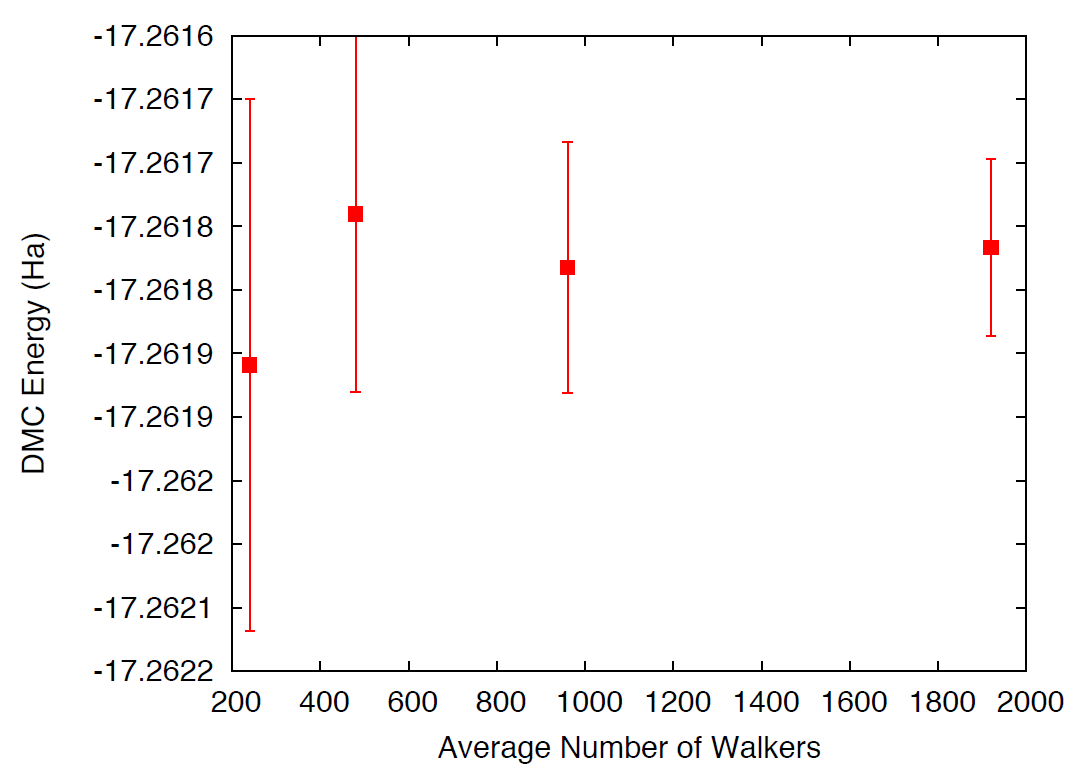
\includegraphics[trim = 0mm 0mm 0mm 0mm, clip,width=0.75\columnwidth]{./figures/lab_advanced_molecules_dmc_popcont.png}
\end{center}
\caption{DMC energy as a function of the average number of walkers.}
\label{fig:lam_dmc_popcont}
\end{figure}

Repeat the same procedure in the other folders by setting (targetWalkers=240,
steps=100, timestep=0.01, blocks=200) in NW240 and (targetWalkers=480, 
steps=100, timestep=0.01, blocks=100) in NW480. When
the simulations complete, use \texttt{qmca} to analyze and plot the energy as a function of the
number of walkers in the calculation. As always, Figure \ref{fig:lam_dmc_popcont} 
shows representative results of the
energy dependence on the number of walkers for a single water molecule. As shown,
less than 240 walkers are needed to obtain an accuracy of 0.1 mHa.


\section{Exercise \#2 Slater-Jastrow wavefunction options}
From this point on in the tutorial we assume familiarity with the basic parameters in the
optimization, VMC, and DMC XML input blocks of QMCPACK. In addition, we assume
familiarity with the submission system. As a result, the folder structure will not contain
any prepared input or submission files, so you will need to generate them using 
input files from exercise 1. In the case of QMCPACK sample 
files, you will find \texttt{optm.xml}, \texttt{vmc dmc.xml}, and \texttt{submit.csh files}. Some of
the options in these files can be left unaltered, but many of them will need to be tailored to
the particular calculation.

In this exercise we will study the dependence of the DMC energy on the choices made
in the wavefunction ansatz. In particular, we will study the influence/dependence of the
VMC energy with the various terms in the Jastrow. We will also study the influence of
the VMC and DMC energies on the SPOs used to form the Slater determinant 
in single-determinant wavefunctions. For this we will use wavefunctions generated
with various exchange-correlation functionals in DFT. Finally, we will optimize a simple
multideterminant wavefunction and study the dependence of the energy on the number of
configurations used in the expansion. All of these exercises will be performed on the water 
molecule at equilibrium.


\subsection{Influence of Jastrow on VMC energy with HF wavefunction}
In this section we will study the dependence of the VMC energy on the various Jastrow
terms (e.g., 1-body, 2-body and 3-body. From the top directory, go to ``\texttt{ex2\_slater-jastrow-wf-options/jastrow.''} 
We will compare the single-determinant VMC energy using a 2-body 
Jastrow term, both 1- and 2-body terms, and finally 1-, 2- and 3-body
terms. Since we are interested in the influence of the Jastrow, we will use the HF orbitals
calculated in exercise \#1. Make three folders named 2j, 12j, and 123j. For both 2j and
12j, %(we have already optimized a wave-function for the 1-2-3J case, so the steps will be
%slightly different in this case)
 copy the input file \texttt{optm.xml} %and the sample submission file
from ``\texttt{ex1\_first-run-hartree-fock/opt.}'' This input file performs both wavefunction optimization 
and a VMC calculation. Remember to correct relative paths to the PP directory. Copy the un-optimized HF \texttt{wavefunction} and \texttt{particleset} files
from ``\texttt{ex1\_first-run-hartree-fock/convert}''; if you followed the instructions in exercise \#1 these should be
named \texttt{h2o.wfs.xml} and \texttt{h2o.ptcl.xml}. Otherwise, you can obtained them from the
REFERENCE files. Modify the \texttt{h2o.wfs.xml} file to remove the appropriate Jastrow
blocks. For example, for a 2-body Jastrow (only), you need to eliminate the Jastrow
blocks named \ixml{<jastrow name="J1"} and \ixml{<jastrow name="J3."} In the case of 12j, remove
only \ixml{<jastrow name="J3."} Recommended settings for the optimization run are nodes=32,
threads=16, blocks=250, samples=128000, time-step=0.5, 8 optimization loops. Recommended settings in the
VMC section are walkers=16, blocks=1000, steps=1, substeps=100. Notice that
samples should always be set to blocks*threads per node*nodes = 32*16*250=128000. Repeat 
the process in both 2j and 12j cases. For the 123j case, the wavefunction has
already been optimized in the previous exercise. Copy the optimized HF wavefunction and
the particleset from ``\texttt{ex1\_first-run-hartree-fock/opt.}'' Copy the input file from any of the previous runs and remove the optimization block from the
input, just leave the VMC step. In all three cases, modify the submission script and submit the run.

\begin{figure}
\begin{center}
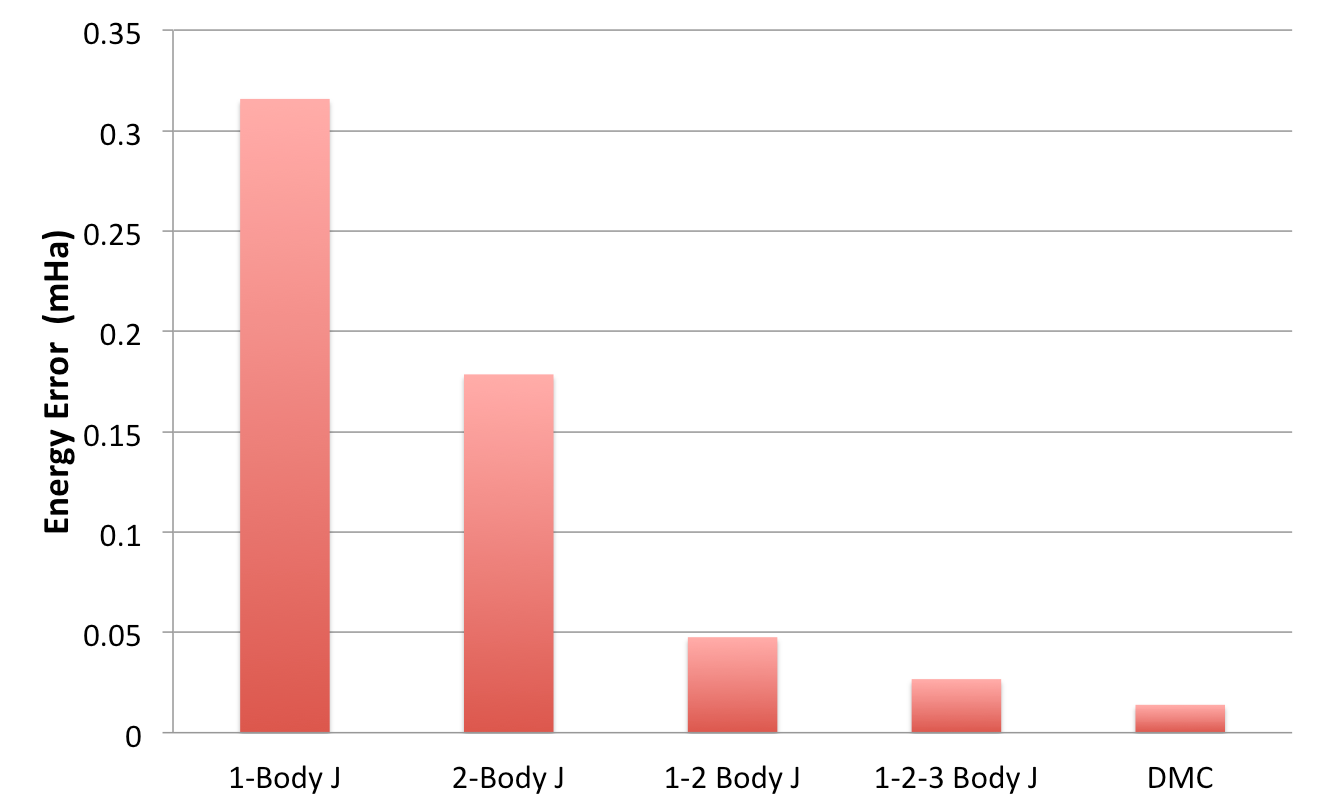
\includegraphics[trim = 0mm 0mm 0mm 0mm, clip,width=0.75\columnwidth]{./figures/lab_advanced_molecules_vmc_jastrow.png}
\end{center}
\caption{VMC energy as a function of Jastrow type.}
\label{fig:lam_vmc_jastrow}
\end{figure}

Because these simulations will take several minutes to complete, this is an excellent opportunity
to go to Section~\ref{sec:lab_adv_mol_wf_appendix}, ``Appendix E: Wavefunction XML block," and review the wavefunction XML block used by QMCPACK. When the
simulations are completed, use \texttt{qmca} to analyze the output files. Using your favorite plotting
program (e.g., gnu plot), plot the energy and variance as a function of the Jastrow form.
Figure \ref{fig:lam_vmc_jastrow} shows a typical result for this calculation. As can be seen, the VMC energy and
variance depends strongly on the form of the Jastrow. Since the DMC error bar is directly
related to the variance of the VMC energy, improving the Jastrow will always lead to a
reduction in the DMC effort. In addition, systematic approximations (time step, number of
walkers, etc.) are also reduced with improved wavefunctions.


\subsection{Generation of wavefunctions from DFT using GAMESS}
In this section we will use GAMESS to generate wavefunctions for QMCPACK from
DFT calculations. From the top folder, go to ``\texttt{ex2\_slater-jastrow-wf-options/orbitals}.'' To demonstrate
the variation in DMC energies with the choice of DFT orbitals, we will choose the following
set of exchange-correlation functionals (PBE, PBE0, BLYP, B3LYP). For each functional,
make a directory using your preferred naming convention (e.g., the name of the functional).
Go into each folder and copy a GAMESS input file from %for a ROHF calculation from
``\texttt{ex1\_first-run-hartree-fock/gms}.'' %, a file named rohf.inp should exist.
 Rename the file with your preferred naming convention; we suggest using \texttt{h2o.[dft].inp}, where [dft] is the name of
the functional used in the calculation. At this point, this input file should be identical to the
one used to generate the HF wavefunction in exercise \#1. To perform a DFT
calculation we only need to add ``DFTTYP'' to the \igamess{\$CONTRL ... \$END} section and set
it to the desired functional type, for example, ``DFTTYP=PBE'' for a PBE functional. This
variable must be set to (PBE, PBE0, BLYP, B3LYP) to obtain the appropriate functional in
GAMESS. For a complete list of implemented functionals, see the GAMESS input manual.


\subsection{Optimization and DMC calculations with DFT wavefunctions}
In this section we will optimize the wavefunction generated in the previous step and
perform DMC calculations. From the top directory, go to “\texttt{ex2\_slater-jastrow-wf-options/orbitals}.”
The steps required to achieve this are identical to those used to optimize the wavefunction
with HF orbitals. Make individual folders for each calculation and obtain the necessary files
to perform optimization, for example, VMC and DMC calculations from ``for \texttt{ex1\_first-run-hartree-fock/opt}'' and ``\texttt{ex1\_first-run-hartree-fock/dmc\_ts}.''
%A file named optm vmc dmc.xml should exist that contains all three execution blocks. 
For each functional, make the appropriate modifications to the input files and copy the \texttt{particleset} and \texttt{wavefunction} files from the appropriate directory in “\texttt{ex2\_slater-jastrow-wf-options/orbitals/[dft]}.” We
recommend the following settings: nodes=32, threads=16, (in optimization) blocks=250,
samples=128000, timestep=0.5, 8 optimization loops, (in VMC) walkers=16, blocks=100,
steps=1, substeps=100, (in DMC) blocks 400, targetWalkers=960, and timestep=0.01. Submit
the runs and analyze the results using \texttt{qmca}.

How do the energies compare against each other? How do they compare against DMC
energies with HF orbitals?
%Orbital Sets and Configurations in 
\section{Exercise \#3: Multideterminant wavefunctions}
In this exercise we will study the dependence of the DMC energy on the set of orbitals
and the type of configurations included in a multideterminant wavefunction. 

\subsection{Generation of a CISD wavefunctions using GAMESS}
In this section we will use GAMESS to generate a multideterminant wavefunction with
configuration interaction with single and double excitations (CISD). In CISD, the Schrodinger equation is solved exactly on a basis of determinants 
including the HF determinant and all its single and double excitations. 

Go to ``\texttt{ex3\_multi-slater-jastrow/cisd/gms}'' and you will see input and output files named \texttt{h2o.cisd.inp} and \texttt{h2o.cisd.out}. Because of technical problems with GAMESS in the BGQ architecture of VESTA, we are unable to use CISD properly in GAMESS. Consequently, the output of the calculation is already provided in the directory. 

%You'll see several input and output files named h2o.XXX.inp
%and h2o.XXX.out, where XXX is one of the following multi-determinant methods: CISD,
%CASSCF, CASCI, SOCI. 

There will be time in the next step to study the GAMESS input
files and the description in Section~\ref{sec:lab_adv_mol_gamess}, ``Appendix A: GAMESS input." %In the next exercise we will use the CISD output, in
%the next exercise we will use the remaining files. 
Since the output is already provided, the
only action needed is to use the converter to generate the appropriate QMCPACK files.  %Copy a submission script from GAMESS/Generic Files and execute the converter for all the output 
%files in the directory (with the exception of CASSCF, which is used to generate orbitals).
%but it doesn’t contain appropriate CI coefficients). 
\begin{shade}
jobrun_vesta convert4qmc h2o.cisd.out -ci h2o.cisd.out \
-readInitialGuess 57 -threshold 0.0075
\end{shade}

We used the PRTMO=.T. flag in the GUESS section to include orbitals in the output file. You should read these orbitals from the output (-readInitialGuess 40).
The highest occupied orbital in any determinant should be 34, so reading 40 orbitals is a safe choice. In this case, it is important to rename the XML files with meaningful names, for example, \texttt{h2o.cisd.wfs.xml}. A threshold of 0.0075 is sufficient for the calculations in the training.


\subsection{Optimization of a multideterminant wavefunction}

In this section we will optimize the wavefunction generated in the previous step. There
is no difference in the optimization steps if a single determinant and a multideterminant wavefunction.
QMCPACK will recognize the presence of a multideterminant wavefunction and will automatically 
optimize the linear coefficients by default. Go to ``\texttt{ex3\_multi-slater-jastrow/cisd}'' and make a folder called 
\texttt{thres0.01}. Copy the \texttt{particleset} and \texttt{wavefunction} files created in the previous step to the current 
directory. With your favorite text editor, open the \texttt{wavefunction} file \texttt{h2o.wfs.xml}. Look for 
the multideterminant XML block and change the ``cutoff'' parameter in detlist to 0.01. Then follow 
the same steps used in Section 9.4.3, ``Optimization and DMC calculations with DFT wavefunctions''
to optimize the wavefunction. Similar to this case, design a QMCPACK input file that performs
wavefunction optimization followed by VMC and DMC calculations. Submit the calculation.

This is a good time to review the GAMESS input file description in Section~\ref{sec:lab_adv_mol_gamess}, ``Appendix A. GAMESS input."
When the run is completed, go to the previous directory and make a new folder named
\texttt{thres0.0075}. Repeat the previous steps to optimize the wavefunction with a cutoff of 0.01, but use a cutoff of 0.0075 this time. This will increase the number of determinants used in the calculation. Notice that the ``cutoff'' parameter in the XML should be less than the ``-threshold 0.0075'' flag passed to the converted, which is further bounded by the PRTTOL flag in the GAMESS input.

After the wavefunction is generated, we are ready to optimize. Instead of starting from an un-optimized wavefunction, we can start from the optimized wavefunction from thres0.01 to speed up convergence. You will need to modify the file and change the cutoff in detlist to 0.0075 with a text editor. Repeat the optimization steps and submit the calculation.

\begin{figure}
\begin{center}
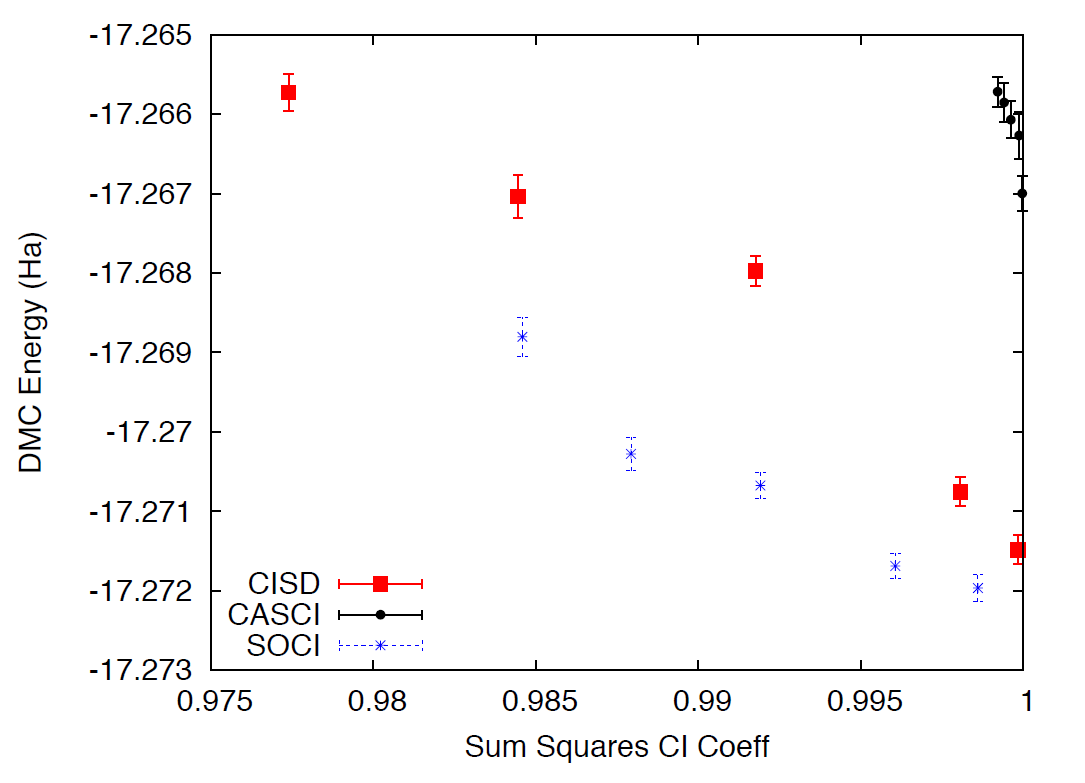
\includegraphics[trim = 0mm 0mm 0mm 0mm, clip,width=0.75\columnwidth]{./figures/lab_advanced_molecules_dmc_ci_cisd.png}
\end{center}
\caption{DMC energy as a function of the sum of the square of CI coefficients from CISD.}
\label{fig:lam_dmc_ci_cisd}
\end{figure}

When you are done, use \texttt{qmca} to analyze the results. Compare the energies at these two
coefficient cutoffs with the energies obtained with DFT orbitals. Because of the time limitations of this tutorial, it is not practical to optimize the wavefunctions with a smaller cutoff since this would require more samples and longer runs due to the larger number of optimizable parameters. Figure \ref{fig:lam_dmc_ci_cisd} shows the results of such exercise: the DMC energy as a function of the cutoff in the wavefunction. As can be seen, a large improvement in the energy is obtained as the number of configurations is increased.


%Since the un-optimized wave-functions were generated in subsection “Generation of a CISD wavefunctions 
%using GAMESS” of exercise \#2, we can skip this section and go straight to the
%wave-function optimization. 

\subsection{CISD, CASCI, and SOCI}

Go to “\texttt{ex3\_multi-slater-jastrow}” and inspect the folders for the remaining wavefunction types: CASCI and SOCI. Follow the steps in the previous exercise and obtain the optimized wavefunctions for these determinant choices. Notice that the SOCI GAMESS output is not included because it is large. Already converted XML inputs can be found in ``\texttt{ex3\_multi-slater-jastrow/soci/thres*}.'' %The exercise has already been performed with a CISD wave-function in exercise \#2.

A CASCI wavefunction is produced from a CI calculation that includes all the determinants 
in a complete active space (CAS) calculation, in this case using the orbitals from a previous CASSCF
calculation. In this case we used a CAS(8,8) active space that includes all determinants
generated by distributing 8 electrons in the lowest 8 orbitals. A SOCI calculation is similar
to the CAS-CI calculation, but in addition to the determinants in the CAS it also includes
all single and double excitations from all of them, leading to a much larger determinant
set. Since you now have considerable experience optimizing wavefunctions and calculating
DMC energies, we will leave it to you to complete the remaining tasks on your own.
If you need help, refer to previous exercises in the tutorial. Perform optimizations for both
wavefunctions using cutoffs in the CI expansion of 0.01 an 0.0075. If you have time, try to optimize the wavefunctions with a cutoff of 0.005. Analyze the results and plot
the energy as a function of cutoff for all three cases: CISD, CAS-CI, and SOCI.

Figure  \ref{fig:lam_dmc_ci_cisd} shows the result of similar calculations using more samples and smaller cutoffs.
The results should be similar to those produced in the tutorial. For reference, the exact
energy of the water molecule with ECPs is approximately -17.276 Ha. From the results of the
tutorial, how does the selection of determinants relate to the expected DMC energy?
What about the choice in the set of orbitals?


\newpage
\section{Appendix A: GAMESS input}\label{sec:lab_adv_mol_gamess}
In this section we provide a brief description of the GAMESS input needed to produce
trial wavefunction for QMC calculations with QMCPACK. We assume basic familiarity
with GAMESS input structure, particularly regarding the input of atomic coordinates and
the definition of Gaussian basis sets. This section focuses on generation of the output
files needed by the converter tool, \texttt{convert4qmc}. For a description of the converter, see Section~\ref{sec:lab_adv_mol_convert4qmc}, ``Appendix B: convert4qmc."

Only a subset of the methods available in GAMESS can be used to generate wavefunctions 
for QMCPACK, and we restrict our description to these.
For a complete description of all the options and methods available
in GAMESS, please refer to the official documentation at ``http://www.msg.ameslab.gov/gamess/documentation.html.”

Currently, \texttt{convert4qmc} can process output for the following methods in GAMESS (in
SCFTYP): RHF, ROHF, and MCSCF. Both HF and DFT calculations (any DFT
type) can be used in combination with RHF and ROHF calculations. For MCSCF and CI
calculations, ALDET, ORMAS, and GUGA drivers can be used (details follow).


\subsection{HF input}
The following input will perform a restricted HF calculation on a closed-shell singlet 
(multiplicity=1). This will generate RHF orbitals for any molecular system defined in 
\ishell{\$DATA ... \$END}.

\begin{lstlisting}[style=GAMESS]
$CONTRL SCFTYP=RHF RUNTYP=ENERGY MULT=1
ISPHER=1 EXETYP=RUN COORD=UNIQUE MAXIT=200 $END
$SYSTEM MEMORY=150000000 $END
$GUESS GUESS=HUCKEL $END
$SCF DIRSCF=.TRUE. $END
$DATA
...
Atomic Coordinates and basis set
...
$END
\end{lstlisting}

Main options:
\begin{enumerate}
  \item{SCFTYP: Type of SCF method, options: RHF, ROHF, MCSCF, UHF and NONE.}
  \item{RUNTYP: Type of run. For QMCPACK wavefunction generation this should always be ENERGY.}
  \item{MULT: Multiplicity of the molecule.}
  \item{ISPHER: Use spherical harmonics (1) or Cartesian basis functions (-1).}
  \item{COORD: Input structure for the atomic coordinates in \$DATA.}
\end{enumerate}


\subsection{DFT calculations}
The main difference between the input for a RHF/ROHF calculation and a DFT calculation 
is the definition of the DFTTYP parameter. If this is set in the \$CONTROL
section, a DFT calculation will be performed with the appropriate functional. Notice that
although the default values are usually adequate, DFT calculations have many options involving
the integration grids and accuracy settings. Make sure you study the input manual to be
aware of these. Refer to the input manual for a list of the implemented exchange-correlation
functionals.


\subsection{MCSCF}
MCSCF calculations are performed by setting SCFTYP=MCSCF in the CONTROL
section. If this option is set, an MCSCF section must be added to the input file with the
options for the calculation. An example section for the water molecule used in the tutorial
follows.

\begin{lstlisting}[style=GAMESS]
$MCSCF CISTEP=GUGA MAXIT=1000 FULLNR=.TRUE. ACURCY=1.0D-5 $END
\end{lstlisting}

The most important parameter is CISTEP, which defines the CI package used. The only
options compatible with QMCPACK are: ALDET, GUGA, and ORMAS. Depending on the
package used, additional input sections are needed.


\subsection{CI}
Configuration interaction (full CI, truncated CI, CAS-CI, etc) calculations are performed
by setting \igamess{SCFTYP=NONE} and \igamess{CITYP=GUGA,ALDET,ORMAS}. Each one of these packages 
requires further input sections, which are typically slightly different from the input sections
needed for MCSCF runs.


\subsection{GUGA: Unitary group CI package}
The GUGA package is the only alternative if one wants CSFs with GAMESS. We subsequently provide a very brief description of the input sections needed to perform MCSCF, CASCI,
truncated CI, and SOCI with this package. For a complete description of these methods and
all the options available, please refer to the GAMESS input manual.

\subsubsection{GUGA-MCSCF}
The following input section performs a CASCI calculation with a CAS that includes 8
electrons in 8 orbitals (4 DOC and 4 VAL), for example, CAS(8,8). NMCC is the number of frozen
orbitals (doubly occupied orbitals in all determinants), NDOC is the number of double
occupied orbitals in the reference determinant, NVAL is the number of singly occupied
orbitals in the reference (for spin polarized cases), and NVAL is the number of orbitals in
the active space. Since FORS is set to .TRUE., all configurations in the active space will
be included. ISTSYM defines the symmetry of the desired state.

\begin{lstlisting}[style=GAMESS]
$MCSCF CISTEP=GUGA MAXIT=1000 FULLNR=.TRUE. ACURCY=1.0D-5 $END
$DRT GROUP=C2v NMCC=0 NDOC=4 NALP=0 NVAL=4 ISTSYM=1 MXNINT= 500000 FORS=.TRUE. $END
\end{lstlisting}

\subsubsection{GUGA-CASCI}
The following input section performs a CASCI calculation with a CAS that includes 8
electrons in 8 orbitals (4 DOC and 4 VAL), for example, CAS(8,8). NFZC is the number of frozen
orbitals (doubly occupied orbitals in all determinants). All other parameters are identical
to those in the MCSCF input section.

\begin{lstlisting}[style=GAMESS]
$CIDRT GROUP=C2v NFZC=0 NDOC=4 NALP=0 NVAL=4 NPRT=2 ISTSYM=1 FORS=.TRUE. MXNINT= 500000 $END
$GUGDIA PRTTOL=0.001 CVGTOL=1.0E-5 ITERMX=1000 $END
\end{lstlisting}

\subsubsection{GUGA-truncated CI}
The following input sections will lead to a truncated CI calculation. In this particular case
it will perform a CISD calculation since IEXCIT is set to 2. Other values in IEXCIT will lead
to different CI truncations; for example, IEXCIT=4 will lead to CISDTQ. Notice that only
the lowest 30 orbitals will be included in the generation of the excited determinants in this
case. For a full CISD calculation, NVAL should be set to the total number of virtual orbitals.

\begin{lstlisting}[style=GAMESS]
$CIDRT GROUP=C2v NFZC=0 NDOC=4 NALP=0 NVAL=30 NPRT=2 ISTSYM=1 IEXCIT=2 MXNINT= 500000 $END
$GUGDIA PRTTOL=0.001 CVGTOL=1.0E-5 ITERMX=1000 $END
\end{lstlisting}

\subsubsection{GUGA-SOCI}
The following input section performs a SOCI calculation with a CAS that includes 8
electrons in 8 orbitals (4 DOC and 4 VAL), for example, CAS(8,8). Since SOCI is set to .TRUE.,
all single and double determinants from all determinants in the CAS(8,8) will be included.

\begin{lstlisting}[style=GAMESS]
$CIDRT GROUP=C2v NFZC=0 NDOC=4 NALP=0 NVAL=4 NPRT=2 ISTSYM=1 SOCI=.TRUE. NEXT=30 MXNINT= 500000 $END
$GUGDIA PRTTOL=0.001 CVGTOL=1.0E-5 ITERMX=1000 $END
\end{lstlisting}


\subsection{ECP}
To use ECPs in GAMESS, you must define a \{\ishell{\$ECP ... \$END}\} 
block. There must be a definition of a potential for every atom in the system, including
symmetry equivalent ones. In addition, they must appear in the particular order expected
by GAMESS. The following example shows an ECP input block for a single water molecule using
BFD ECPs. To turn on the use of ECPs, the option “ECP=READ” must be added to the
CONTROL input block.

\begin{lstlisting}[style=GAMESS]
$ECP
O-QMC GEN 2 1
3
6.00000000 1 9.29793903
55.78763416 3 8.86492204
-38.81978498 2 8.62925665
1
38.41914135 2 8.71924452
H-QMC GEN 0 0
3
1.000000000000 1 25.000000000000
25.000000000000 3 10.821821902641
-8.228005709676 2 9.368618758833
H-QMC
$END
\end{lstlisting}


\newpage
\section{Appendix B: convert4qmc}\label{sec:lab_adv_mol_convert4qmc}
To generate the particleset and wavefunction XML blocks required by QMCPACK in
calculations with molecular systems, the converter \texttt{convert4qmc} must be used. The converter
will read the standard output from the appropriate quantum chemistry calculation and will
generate all the necessary input for QMCPACK. In the following, we describe the main options of the
converter for GAMESS output. In general, there are three ways to use the converter depending
on the type of calculation performed. The minimum syntax for each option is shown subsequently.
For a description of the XML files produced by the converter, see Section~\ref{sec:lab_adv_mol_wf_appendix}, ``Appendix E: Wavefunction XML block."

\begin{enumerate}
  \item{For all single-determinant calculations (HF and DFT with any DFTTYP):}
  \begin{shade}
convert4qmc -gamessAscii single det.out
  \end{shade}
  \begin{itemize}
    \item{single det.out is the standard output generated by GAMESS.}
  \end{itemize}
  \item{\textit{(This option is not recommended. Use the following option to avoid mistakes.)} For 
    multideterminant calculations where the orbitals and configurations are read from different
    files (e.g., when using orbitals from a MCSCF run and configurations from a
    subsequent CI run):}
  \begin{shade}
convert4qmc -gamessAscii orbitals multidet.out -ci cicoeff multidet.out
  \end{shade}
  \begin{itemize}
    \item{orbitals\_multidet.out is the standard output from the calculation that generates the
       orbitals. cicoeff multidet.out is the standard output from the calculation that calculates 
       the CI expansion.}
  \end{itemize}
  \item{For multideterminant calculations where the orbitals and configurations are read from
    the same file, using PRTMO=.T. in the GUESS input block:}
  \begin{shade}
convert4qmc -gamessAscii multi det.out -ci multi det.out -readInitialGuess Norb
  \end{shade}
  \begin{itemize}
    \item{multi\_det.out is the standard output from the calculation that calculates the CI expansion.}
  \end{itemize}
\end{enumerate}

Options:
\begin{itemize}
\item{\textbf{-gamessAscii file.out}: Standard output of GAMESS calculation. With the exception 
of determinant configurations and coefficients in multideterminant calculations,
everything else is read from this file including atom coordinates, basis sets, SPOs, ECPs, number of electrons, multiplicity, etc.}

\item{\textbf{-ci file.out}: In multideterminant calculations, determinant configurations and 
coefficients are read from this file. Notice that SPOs are NOT read
from this file. Recognized CI packages are ALDET, GUGA, and ORMAS. Output
produced with the GUGA package MUST have the option “NPRT=2” in the CIDRT
or DRT input blocks.}

\item{\textbf{-threshold cutoff}: Cutoff in multideterminant expansion. Only configurations with
coefficients above this value are printed.}

\item{\textbf{-zeroCI}: Sets to zero the CI coefficients of all determinants, with the exception of the
first one.}

\item{\textbf{-readInitialGuess Norb}: Reads Norb initial orbitals (“INITIAL GUESS ORBITALS”) 
from GAMESS output. These are orbitals generated by the GUESS input
block and printed with the option “PRTMO=.T.”. Notice that this is useful only in
combination with the option “GUESS=MOREAD” and in cases where the orbitals
are not modified in the GAMESS calculation, e.g. CI runs. This is the recommended
option in all CI calculations.}

\item{\textbf{-NaturalOrbitals Norb}: Read Norb “NATURAL ORBITALS” from GAMESS
output. The natural orbitals must exists in the output, otherwise the code aborts.}

\item{\textbf{-add3BodyJ}: Adds 3-body Jastrow terms (e-e-I) between electron pairs (both
same spin and opposite spin terms) and all ion species in the system. The radial
function is initialized to zero, and the default cutoff is 10.0 bohr. The converter will
add a 1- and 2-body Jastrow to the wavefunction block by default.}
\end{itemize}

\subsection{Useful notes}
\begin{itemize}
  \item{The type of SPOs read by the converter depends on the type of
calculation and on the options used. By default, when neither -readInitialGuess nor
-NaturalOrbitals are used, the following orbitals are read in each case (notice that
-readInitialGuess or -NaturalOrbitals are mutually exclusive):}
  \begin{itemize}
    \item{RHF and ROHF: “EIGENVECTORS”}
    \item{MCSCF: “MCSCF OPTIMIZED ORBITALS”}
    \item{GUGA, ALDET, ORMAS: Cannot read orbitals without -readInitialGuess or -NaturalOrbitals options.}
  \end{itemize}
  \item{The SPOs and printed CI coefficients in MCSCF calculations are
not consistent in GAMESS. The printed CI coefficients correspond to the next-to-last
iteration; they are not recalculated with the final orbitals. So to get appropriate 
CI coefficients from MCSCF calculations, a subsequent CI (no SCF) calculation
is needed to produce consistent orbitals. In principle, it is possible to read the orbitals 
from the MCSCF output and the CI coefficients and configurations from the
output of the following CI calculations. This could lead to problems in principle since
GAMESS will rotate initial orbitals by default to obtain an initial guess consistent 
with the symmetry of the molecule. This last step is done by default and can
change the orbitals reported in the MCSCF calculation before the CI is performed.
To avoid this problem, we highly recommend using the preceding option \#3 to
read all the information from the output of the CI calculation; this requires the use
of “PRTMO=.T.” in the GUESS input block. Since the orbitals are printed after any
symmetry rotation, the resulting output will always be consistent.}
\end{itemize}


\newpage
\section{Appendix C: Wavefunction optimization XML block}\label{sec:lab_adv_mol_opt_appendix}

\begin{lstlisting}[style=QMCPXML,caption=``Sample XML optimization block.",label=lst:lam_xml_opt]
  <loop max="10">
    <qmc method="linear" move="pbyp" checkpoint="-1" gpu="no">
    <parameter name="blocks">     10  </parameter>
      <parameter name="warmupsteps"> 25 </parameter>
      <parameter name="steps"> 1 </parameter>
      <parameter name="substeps"> 20 </parameter>
      <parameter name="timestep"> 0.5 </parameter>
      <parameter name="samples"> 10240  </parameter>
      <cost name="energy">                   0.95 </cost>
      <cost name="unreweightedvariance">     0.0 </cost>
      <cost name="reweightedvariance">       0.05 </cost>
      <parameter name="useDrift">  yes </parameter>
      <parameter name="bigchange">10.0</parameter>
      <estimator name="LocalEnergy" hdf5="no"/>
      <parameter name="usebuffer"> yes </parameter>
      <parameter name="nonlocalpp"> yes </parameter>
      <parameter name="MinMethod">quartic</parameter>
      <parameter name="exp0">-6</parameter>
      <parameter name="alloweddifference"> 1.0e-5 </parameter>
      <parameter name="stepsize">  0.15 </parameter>
      <parameter name="nstabilizers"> 1 </parameter>
    </qmc>
  </loop>
\end{lstlisting}

Options:
\begin{itemize}
  \item{bigchange: (default 50.0) Largest parameter change allowed}
  \item{usebuffer: (default no) Save useful information during VMC}
  \item{nonlocalpp: (default no) Include nonlocal energy on 1-D min}
  \item{MinMethod: (default quartic) Method to calculate magnitude of parameter change
quartic: fit quartic polynomial to four values of the cost function obtained using reweighting 
along chosen direction linemin: direct line minimization using reweighting rescale:
no 1-D minimization. Uses Umrigars suggestions.}
  \item{stepsize: (default 0.25) Step size in either quartic or linemin methods.}
  \item{alloweddifference: (default 1e-4) Allowed increase in energy}
  \item{exp0: (default -16.0) Initial value for stabilizer (shift to diagonal of H). Actual value
of stabilizer is 10 exp0}
  \item{nstabilizers: (default 3) Number of stabilizers to try}
  \item{stabilizaterScale: (default 2.0) Increase in value of exp0 between iterations.}
  \item{max its: (default 1) Number of inner loops with same sample}
  \item{minwalkers: (default 0.3) Minimum value allowed for the ratio of effective samples
to actual number of walkers in a reweighting step. The optimization will stop if the
effective number of walkers in any reweighting calculation drops below this value. Last
set of acceptable parameters are kept.}
  \item{maxWeight: (defaul 1e6) Maximum weight allowed in reweighting. Any weight above
this value will be reset to this value.}
\end{itemize}

Recommendations:
\begin{itemize}
  \item{Set samples to equal to (\#threads)*blocks.}
  \item{Set steps to 1. Use substeps to control correlation between samples.}
  \item{For cases where equilibration is slow, increase both substeps and warmupsteps.}
  \item{For hard cases (e.g., simultaneous optimization of long MSD and 3-Body J), set exp0
to 0 and do a single inner iteration (max its=1) per sample of configurations.}
\end{itemize}


\newpage
\section{Appendix D: VMC and DMC XML block}\label{sec:lab_adv_mol_vmcdmc_appendix}

\begin{lstlisting}[style=QMCPXML,caption=``Sample XML blocks for VMC and DMC calculations.",label=lst:lam_xml_vmc_dmc]
  <qmc method="vmc" move="pbyp" checkpoint="-1">
    <parameter name="useDrift">yes</parameter>
    <parameter name="warmupsteps">100</parameter>
    <parameter name="blocks">100</parameter>
    <parameter name="steps">1</parameter>
    <parameter name="substeps">20</parameter>
    <parameter name="walkers">30</parameter>
    <parameter name="timestep">0.3</parameter>
    <estimator name="LocalEnergy" hdf5="no"/>
  </qmc>
  <qmc method="dmc" move="pbyp" checkpoint="-1">
    <parameter name="nonlocalmoves">yes</parameter>
    <parameter name="targetWalkers">1920</parameter>
    <parameter name="blocks">100</parameter>
    <parameter name="steps">100</parameter>
    <parameter name="timestep">0.1</parameter>
    <estimator name="LocalEnergy" hdf5="no"/>
  </qmc>
\end{lstlisting}

General Options:
\begin{itemize}
\item{\textbf{move}: (default ``walker”) Type of electron move. Options: ``pbyp” and ``walker.”}
\item{\textbf{checkpoint}: (default ``-1”) (If > 0) Generate checkpoint files with given frequency.
The calculations can be restarted/continued with the produced checkpoint files.}
\item{\textbf{useDrift}: (default ``yes”) Defines the sampling mode. useDrift = ``yes” will
use Langevin acceleration to sample the VMC and DMC distributions, while
useDrift=``no” will use random displacements in a box.}
\item{\textbf{warmupSteps}: (default 0) Number of steps warmup steps at the beginning of the
calculation. No output is produced for these steps.}
\item{\textbf{blocks}: (default 1) Number of blocks (outer loop).}
\item{\textbf{steps}: (default 1) Number of steps per blocks (middle loop).}
\item{\textbf{sub steps}: (default 1) Number of substeps per step (inner loop). During substeps,
the local energy is not evaluated in VMC calculations, which leads to faster execution.
In VMC calculations, set substeps to the average autocorrelation time of the desired
quantity.}
\item{\textbf{time step}: (default 0.1) Electronic time step in bohr.}
\item{\textbf{samples}: (default 0) Number of walker configurations saved during the current 
calculation.}
\item{\textbf{walkers}: (default \#threads) In VMC, sets the number of walkers per node. The total
number of walkers in the calculation will be equal to walkers*(\# nodes).}
\end{itemize}

Options unique to DMC:
\begin{itemize}
\item{\textbf{targetWalkers}: (default \#walkers from previous calculation, e.g., VMC). Sets the
target number of walkers. The actual population of walkers will fluctuate around this
value. The walkers will be distributed across all the nodes in the calculation. On a
given node, the walkers are split across all the threads in the system.}
\item{\textbf{nonlocalmoves}: (default ``no”) Set to ``yes” to turns on the use of Casula’s T-moves.}
\end{itemize}


\newpage
\section{Appendix E: Wavefunction XML block}\label{sec:lab_adv_mol_wf_appendix}

\begin{lstlisting}[style=QMCPXML,caption=``Basic framework for a single-determinant determinantset XML block.",label=lst:lam_xml_determinantset]
<wavefunction name="psi0" target="e">
  <determinantset type="MolecularOrbital" name="LCAOBSet"
   source="ion0" transform="yes">
    <basisset name="LCAOBSet">
      <atomicBasisSet name="Gaussian-G2" angular="cartesian" type="Gaussian" elementType="O" normalized="no">
      ...
      </atomicBasisSet>
    </basisset>
    <slaterdeterminant>
      <determinant id="updet" size="4">
        <occupation mode="ground"/>
        <coefficient size="57" id="updetC">
        ...
        </coefficient>
      </determinant>
      <determinant id="downdet" size="4">
        <occupation mode="ground"/>
        <coefficient size="57" id="downdetC">
        ...
        </coefficient>
      </determinant>
    </slaterdeterminant>

  </determinantset>

  <jastrow name="J2" type="Two-Body" function="Bspline" print="yes">
  ...
  </jastrow>

</wavefunction>
\end{lstlisting}

In this section we describe the basic format of a QMCPACK wavefunction XML block.
Everything listed in this section is generated by the appropriate converter tools. Little to
no modification is needed when performing standard QMC calculations. As a result, this
section is meant mainly for illustration purposes. Only experts should attempt to modify
these files (with very few exceptions like the cutoff of CI coefficients and the cutoff in Jastrow
functions) since changes can lead to unexpected results.

A QMCPACK wavefunction XML block is a combination of a determinantset, which
contains the antisymmetric part of the wavefunction and one or more Jastrow blocks.
The syntax of the antisymmetric block depends on whether the wavefunction is a single
determinant or a multideterminant expansion. Listing \ref{lst:lam_xml_determinantset} 
shows the general structure of the
single-determinant case. The determinantset block is composed of a basisset block, which
defines the atomic orbital basis set, and a slaterdeterminant block, which defines the SPOs and occupation numbers of the Slater determinant.
% Listing \ref{lst:lam_xml_basisset} 
%shows a section
%of a basisset block for a gold atom. The structure of this block is rigid and should not
%be modified.
 Listing \ref{lst:lam_xml_slaterdeterminant} shows a (piece of a) sample of a 
slaterdeterminant block. The
slaterdeterminant block consists of two determinant blocks, one for each electron spin. The
parameter ``size” in the determinant block refers to the number of SPOs
present while the ``size” parameter in the coefficient block refers to the number of atomic
basis functions per SPO.

\begin{lstlisting}[style=QMCPXML,caption=``Sample XML block for the single Slater determinant case.",label=lst:lam_xml_slaterdeterminant]
      <slaterdeterminant>
        <determinant id="updet" size="5">
          <occupation mode="ground"/>
          <coefficient size="134" id="updetC">
  9.55471000000000e-01 -3.87000000000000e-04  6.51140000000000e-02  2.17700000000000e-03
  1.43900000000000e-03  4.00000000000000e-06 -4.58000000000000e-04 -5.20000000000000e-05
 -2.40000000000000e-05  6.00000000000000e-06 -0.00000000000000e+00 -0.00000000000000e+00
 -0.00000000000000e+00 -0.00000000000000e+00 -0.00000000000000e+00 -0.00000000000000e+00
 -0.00000000000000e+00 -0.00000000000000e+00 -0.00000000000000e+00 -0.00000000000000e+00
 -0.00000000000000e+00 -0.00000000000000e+00 -0.00000000000000e+00 -0.00000000000000e+00
 -0.00000000000000e+00 -0.00000000000000e+00 -0.00000000000000e+00 -0.00000000000000e+00
 -0.00000000000000e+00 -0.00000000000000e+00 -0.00000000000000e+00 -0.00000000000000e+00
 -0.00000000000000e+00 -0.00000000000000e+00 -0.00000000000000e+00 -0.00000000000000e+00
 -0.00000000000000e+00 -5.26000000000000e-04  2.63000000000000e-04  2.63000000000000e-04
 -0.00000000000000e+00 -0.00000000000000e+00 -0.00000000000000e+00 -1.27000000000000e-04
  6.30000000000000e-05  6.30000000000000e-05 -0.00000000000000e+00 -0.00000000000000e+00
 -0.00000000000000e+00 -3.20000000000000e-05  1.60000000000000e-05  1.60000000000000e-05
 -0.00000000000000e+00 -0.00000000000000e+00 -0.00000000000000e+00  7.00000000000000e-06
\end{lstlisting}
Listing \ref{lam_xml_multideterminant} shows the general structure of the multideterminant case. 
Similar to the
single-determinant case, the determinantset must contain a basisset block. This definition is
identical to the one described previously. In this case, the definition of the SPOs
must be done independently from the definition of the determinant configurations; the latter
is done in the sposet block, while the former is done on the multideterminant block. Notice
that two sposet sets must be defined, one for each electron spin. The name of each sposet set
is required in the definition of the multideterminant block. The determinants are defined in
terms of occupation numbers based on these orbitals.

\begin{lstlisting}[style=QMCPXML,caption=``Basic framework for a multideterminant determinantset XML block.",label=lam_xml_multideterminant]
  <wavefunction id="psi0" target="e">
    <determinantset name="LCAOBSet" type="MolecularOrbital" transform="yes" source="ion0">
      <basisset name="LCAOBSet">
        <atomicBasisSet name="Gaussian-G2" angular="cartesian" type="Gaussian" elementType="O" normalized="no">
        ...
        </atomicBasisSet>
        ...
      </basisset>
      <sposet basisset="LCAOBSet" name="spo-up" size="8">
        <occupation mode="ground"/>
        <coefficient size="40" id="updetC">
        ...
</coefficient>
      </sposet>
      <sposet basisset="LCAOBSet" name="spo-dn" size="8">
        <occupation mode="ground"/>
        <coefficient size="40" id="downdetC">
        ...
      </coefficient>
      </sposet>
      <multideterminant optimize="yes" spo_up="spo-up" spo_dn="spo-dn">
        <detlist size="97" type="CSF" nca="0" ncb="0" nea="4" neb="4" nstates="8" cutoff="0.001">
          <csf id="CSFcoeff_0" exctLvl="0" coeff="0.984378" qchem_coeff="0.984378" occ="22220000">
            <det id="csf_0-0" coeff="1" alpha="11110000" beta="11110000"/>
          </csf>
          ...
        </detlist>
      </multideterminant>
    </determinantset>
    <jastrow name="J2" type="Two-Body" function="Bspline" print="yes">
    ...
    </jastrow>
  </wavefunction>
\end{lstlisting}

There are various options in the multideterminant block that users should be aware of.
\begin{itemize}
  \item{cutoff: (IMPORTANT! ) Only configurations with (absolute value) “qchem coeff”
larger than this value will be read by QMCPACK.}
  \item{optimize: Turn on/off the optimization of linear CI coefficients.}
  \item{coeff: (in csf ) Current coefficient of given configuration. Gets updated during 
wavefunction optimization.}
  \item{qchem coeff: (in csf ) Original coefficient of given configuration from GAMESS 
calculation. This is used when applying a cutoff to the configurations read from the file.
The cutoff is applied on this parameter and not on the optimized coefficient.}
  \item{nca and nab: Number of core orbitals for up/down electrons. A core orbital is an
orbital that is doubly occupied in all determinant configurations, not to be confused
with core electrons. These are not explicitly listed on the definition of configurations.}
  \item{nea and neb: Number of up/down active electrons (those being explicitly correlated).}
  \item{nstates: Number of correlated orbitals}.
  \item{size (in detlist ): Contains the number of configurations in the list.}
\end{itemize}
The remaining part of the determinantset block is the definition of Jastrow factor. Any
number of these can be defined. Figure \ref{fig:lam_xml_jastrow} shows a sample Jastrow 
block including 1-, 2- and 3-body terms. This is the standard block produced by 
\texttt{convert4qmc} with the option -add3BodyJ (this particular example is for a water molecule). 
Optimization of individual radial functions can be turned on/off using the “optimize” 
parameter. It can be added to any coefficients block, even though it is currently not 
present in the J1 and J2 blocks.

\begin{lstlisting}[style=QMCPXML,caption=``Sample Jastrow XML block.",label=fig:lam_xml_jastrow]
<jastrow name="J2" type="Two-Body" function="Bspline" print="yes">
      <correlation rcut="10" size="10" speciesA="u" speciesB="u">
        <coefficients id="uu" type="Array">0.0 0.0 0.0 0.0 0.0 0.0 0.0 0.0 0.0 0.0</coefficients>
      </correlation>
      <correlation rcut="10" size="10" speciesA="u" speciesB="d">
        <coefficients id="ud" type="Array">0.0 0.0 0.0 0.0 0.0 0.0 0.0 0.0 0.0 0.0</coefficients>
      </correlation>
    </jastrow>
    <jastrow name="J1" type="One-Body" function="Bspline" source="ion0" print="yes">
      <correlation rcut="10" size="10" cusp="0" elementType="O">
        <coefficients id="eO" type="Array">0.0 0.0 0.0 0.0 0.0 0.0 0.0 0.0 0.0 0.0</coefficients>
      </correlation>
      <correlation rcut="10" size="10" cusp="0" elementType="H">
        <coefficients id="eH" type="Array">0.0 0.0 0.0 0.0 0.0 0.0 0.0 0.0 0.0 0.0</coefficients>
      </correlation>
    </jastrow>
    <jastrow name="J3" type="eeI" function="polynomial" source="ion0" print="yes">
      <correlation ispecies="O" especies="u" isize="3" esize="3" rcut="10">
        <coefficients id="uuO" type="Array" optimize="yes">
        </coefficients>
      </correlation>
      <correlation ispecies="O" especies1="u" especies2="d" isize="3" esize="3" rcut="10">
        <coefficients id="udO" type="Array" optimize="yes">
        </coefficients>
      </correlation>
      <correlation ispecies="H" especies="u" isize="3" esize="3" rcut="10">
        <coefficients id="uuH" type="Array" optimize="yes">
        </coefficients>
      </correlation>
      <correlation ispecies="H" especies1="u" especies2="d" isize="3" esize="3" rcut="10">
        <coefficients id="udH" type="Array" optimize="yes">
        </coefficients>
      </correlation>
      </jastrow>
\end{lstlisting}

This training assumes basic familiarity with the UNIX operating system. In particular,
we use simple scripts written in “csh.” In addition, we assume you have obtained
all the necessary files and executables and that the training files are located
at \$\{TRAINING TOP\}.

The goal of this training is not only to familiarize you with the execution and
options in QMCPACK but also to introduce you to important concepts in QMC calculations and many-body electronic structure calculations.



%%% Local Variables:
%%% mode: latex
%%% TeX-master: "just_labs"
%%% End:
